\documentclass{beamer}
\usepackage{amsmath}
\usepackage{amssymb}
\usepackage{mathrsfs}
\usepackage[LGR,T1]{fontenc}
\newcommand{\textgreek}[1]{\begingroup\fontencoding{LGR}\selectfont#1\endgroup}
\usepackage[utf8]{inputenc}
\usepackage{caption}
\usepackage{graphicx}
\graphicspath{ {tu/} }

\title[MATH 6380 Project 2]{Study on tree-based methods.}
\subtitle{MATH 6380 project 2}
\author[C.Dong, T.C.LO, J.Xia]
{Chenyang,~DONG \and Tsz Cheung,~LO \and Jiacheng,~XIA}
\usetheme{CambridgeUS}
%\usecolortheme{wolverine}
%%%
% The next block of commands puts the table of contents at the 
% beginning of each section and highlights the current section:

\AtBeginSection[]
{
  \begin{frame}
    \frametitle{Table of Contents}
    \tableofcontents[currentsection]
  \end{frame}
}
%
%%%

\begin{document}
\frame{\titlepage}

\begin{frame}
\frametitle{Outline}
\tableofcontents
\end{frame}

\section{Introduction}
\begin{frame}
\frametitle{Studying tree based methods...}
Why did we choose tree-based methods?
\pause
\begin{itemize}
\item We went through several methods.
\pause
\item Tree-based methods are straight-forward and easy to implement.
\pause
\item There are yet many improvement methods.
\pause
\item Studied the method on 3 datasets.
\end{itemize}
\end{frame}

%xia's part
\section{American Crime Dataset}
\begin{frame}
\begin{block}{The dataset}
This dataset and the preprocessing are the same as project 1.
\end{block}
\pause
\begin{exampleblock}{Goal for this dataset}
Do straightforward analysis and compare with Lasso (PJ 1).
\end{exampleblock}
\begin{alertblock}{What we found}
In terms of MSE, simple regression tree(0.11) slightly worse than Lasso(0.06); bagging, random forest and boosting even better(0.04, 0.02).
\end{alertblock}
\end{frame}

\begin{frame}
\frametitle{Visualize the results}
\begin{figure}[h]
  \centering
  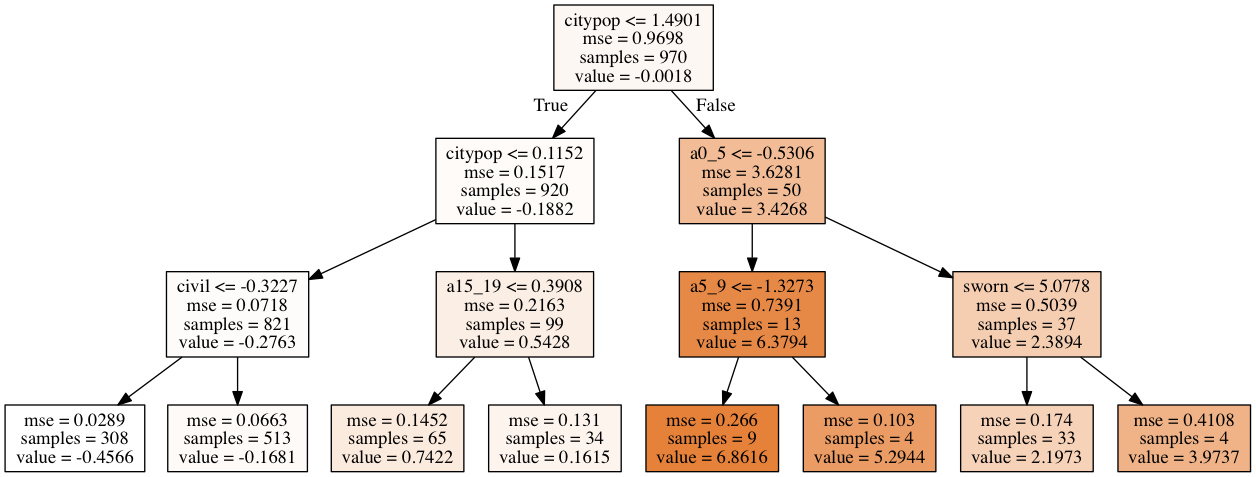
\includegraphics[width=10cm, height=4cm]{crime_treetu}
  \caption{Regression tree on crime data}
\end{figure}
\end{frame}

\begin{frame}
\frametitle{Boosting and random forests}
\begin{figure}
\centering
\begin{minipage}{.5\textwidth}
  \centering
  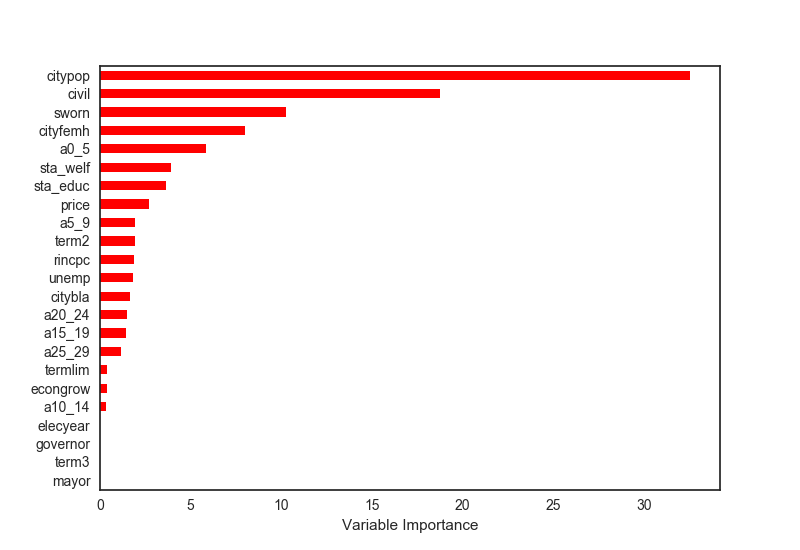
\includegraphics[width=.8\linewidth,height=4cm]{crime_boosttu}
  \captionof{figure}{Importance\\ from boosting}
  \label{fig:test1}
\end{minipage}%
\begin{minipage}{.5\textwidth}
  \centering
  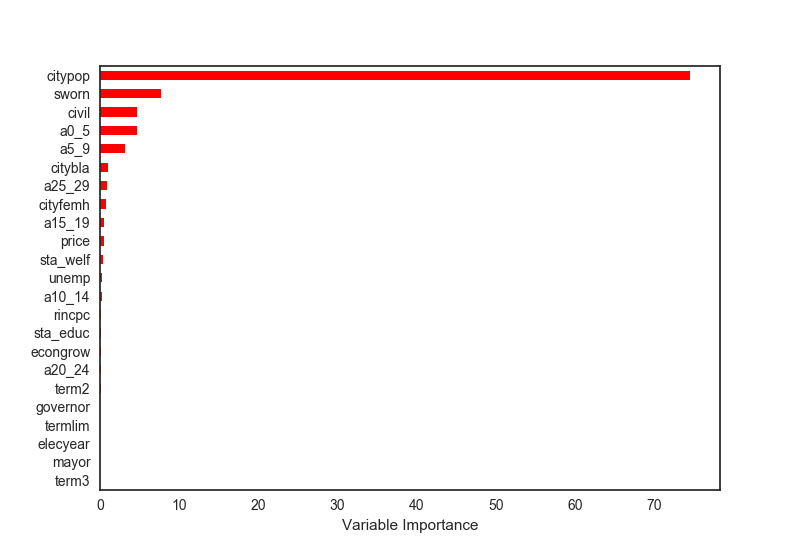
\includegraphics[width=.8\linewidth,height=4cm]{crime_randtu}
  \captionof{figure}{Importance\\ from random forest}
  \label{fig:test2}
\end{minipage}
\end{figure}
\end{frame}

%segfaultdong part
\section{Kaggle 1:  ComboDrug}


%phil's part
\section{Kaggle 2: Binray Drug}
\begin{frame}
\frametitle{Models and Kaggle Results}
Dummy1
\pause
Dummy2
\end{frame}

\begin{frame}
Dummy
\frametitle{Variable Importance}
\end{frame}

\begin{frame}
Dummy
\frametitle{Compared with p-value Selection}
\end{frame}

\begin{frame}
\frametitle{Some Conclusions}
We came up with some conclusions (inferences):
\begin{enumerate}[<+(1)->]
	\item dummy1
	\item dummy2
\end{enumerate}
\end{frame}


%who's part?
\section{Analysis and Conclusion}

\end{document}